\section{Klasické šifry}
V tejto kapitole sa budeme zaoberať históriou a stručným prehľadom klasických šifier.
Spomenieme si aj niektoré základné útoky na klasické šifry. 

\subsection{História}
História klasických šifier a utajovania písomného textu je pravdepodobne tak stará ako samotné písmo.
Písmo, v podobe akej ho poznáme a používame dnes, pravdepodobne pochádza asi spred 3000 rokov pred Kristom a za jeho objaviteľov sa považujú
Feničania.
V niektorých prípadoch predstavovalo už použitie písma utajenie samotného textu.
Príkladom môžu byť Egyptské hieroglyfy alebo klinové písmo používané v Mezopotámii.
Iným príkladom môžu byť semitské jazyky, ktoré sú charakteristické používaním iba spoluhlások bez použitia samohlások,
pretože tie zaviedli až Aremejci a po nich následné Gréci aby pomocou nich boli schopný rozlíšiť jazyky \cite{ks}.
Aj diakritika ako taká má schopnosť rozlišovať významy slov, čo si ale až do 15.storočia nikto nevšímal,
až pokiaľ ju Arabi nezačali používať pri kryptoanalýze rôznych šifier.

Z historického hľadiska nie je možné presne zoradiť ako jednotlivé šifry vznikali, pretože súčasne vznikali na viacerých miestach sveta.
Komunikácia a s ňou spojené sírenie informácii nebolo také rýchle ako dnes, až do roku 1440 keď Johan Guttenberg vynašiel kníhtlač,
čo zjednodušilo výmenu a uchovávanie informácii.
% (TODO: pridať utajovanie informácie)

Ku kryptografii ako aj k rôznym iným vedným disciplínam prispelo v minulosti staré Grécko.
Jedným z najvýznamnejších príspevkov starých Grékov bolo široké rozšírenie abecedy a písomného prejavu.
Gréci písmo prebrali od Feničanov, ktorí na rozdiel od Egypťanov používali jednoduchšie písmo.

V Európe vďaka rozšíreniu abecedy začali vznikať aj prvé šifry, medzi ktoré patrí napríklad Cézarova šifra, ktorá vznikla v Rímskej ríši.
Iným príkladom môže byť transpozičná šifra skytalé, ktorá bola používaná v Sparte.

Pád Rímskej ríše spôsobil úpadok kryptografie, ktorý trval až do obdobia stredoveku. Typickým znakom kryptografie v tomto období bolo
napríklad písanie odzadu, alebo vertikálne, používanie cudzích jazykov, alebo vynechávanie samohlások \cite{ks}.

V stredoveku, kvôli bojom medzi pápežmi Ríma a Avignonu, bola kryptografia zdokonalená a začali sa používať rôzne kódy a nomenklátory.
Ich charakteristickým znakom bolo zamieňanie písmen alebo nahradzovanie mien a titulov osôb v správach.
V tomto období zabezpečovanie utajenia správ pokročilo až na takú úroveň, že na doručovanie správ boli použitý špeciálne vycvičení kuriéri.

V prvej polovici 20. storočia ľudia, ktorí pracovali v oblasti utajovanej komunikácie verili, že na to aby bola zabezpečená utajovaná komunikácia musí byť utajený kľúč a okrem neho aj šifrovací algoritmus. Toto ale odporovalo Kerckhoffovmu princípu, ktorý hovorí že: \textquote{Bezpečnosť šifrovacieho algoritmu musí závisieť výlučne na utajení kľúča a nie algoritmu}. Okrem toho sformuloval aj niekoľko požiadaviek na kryptografický systém, medzi ktoré patria:
\begin{enumerate}
\item systém musí byť teoreticky, alebo aspoň prakticky bezpečný
\item narušenie systému nesmie priniesť ťažkosti odosielateľovi a adresátovi
\item kľúč musí byť ľahko zapamätateľný a ľahko vymeniteľný
\item zašifrovaná správa musí byť prenášateľná telegrafom
\item šifrovacia pomôcka musí byť ľahko prenosná a ovládateľná jedinou osobou
\item systém musí byť jednoduchý, bez dlhého zoznamu pravidiel, nevyžadujúci nadmerné sústredenie
\end{enumerate}
Tieto princípy sú popísané v pôvodnej publikácii od Kerckhoffa \cite{kerckhoff}.

Existovala ale aj iná skupina vedcov, medzi ktorých patril aj Lester S. Hill, ktorý si uvedomoval že kryptológia je úzko spätá z matematikou.
V roku 1941 si na Hillových prácach zakladal A. Adrian Albert, ktorý pochopil, že v šifrovaní je možné použiť viacero algebraických štruktúr.
Neskôr toto všetko usporiadal a zdokonalil Claude E. Shannon, čo možno považovať za ukončenie éry klasických šifier \cite{ks}.

% \todo{Možno pridať/spomenúť steganografiu.}

\subsection{Charakteristika}
Na rozdiel od moderných šifier, ktoré sa používajú dnes, sú tie klasické rozdielne v niektorých hlavných črtách.
Môžeme spomenúť niekoľko:
\begin{itemize}
\item Šifrovanie a dešifrovanie klasickej šifry možno realizovať zväčša pomocou papiera a ceruzky alebo nejakej mechanickej pomôcky.
\item V dnešnej dobe aj vďaka rozšírenému použitiu počítačov stratila väčšina týchto algoritmov svoj význam.
\item Utajuje sa algoritmus a aj kľúč a neuplatňuje sa Kerckhoffov princíp.
\item Na rozdiel od moderných šifier sa používajú malé abecedy.
\item V klasických šifrách je otvorený text, zašifrovaný text a kľúč v abecede reálneho jazyka, pričom v moderných šifrách sa používa binárne kódovanie.
\item Na klasické šifry sa zväčša dá použiť štatistická analýza. 
\end{itemize}
Z spomenutých charakteristík existujú aj výnimky. Napríklad pri Vigenerovej šifre sa algoritmus neutajoval. To platí aj pre Vernamovu šifru, ktorá okrem toho používa navyše binárne znaky. Vernamova šifra je perfektne bezpečná v podľa Shannonovej teórie \cite{ks}.

Klasické šifry môžeme rozdeliť do niekoľkých základných kategórii:
\begin{itemize}

\item \textbf{Substitučné šifry.}
  V prípade že šifra permutuje znaky zdrojovej abecedy, hovoríme o monoalfabetickej šifre.
  Ako príklad môžeme uviesť šifru Atbaš prípadne Cézarovu šifru, alebo iné.
  V inom prípade ak sa aplikuje viacero permutácii podľa polohy znaku v otvorenom texte, tak hovoríme o polyalfabetickej šifre.
  Príkladom je Vigenerova šifra. Ďalším prípadom je polygramová šifra, kde sa z otvoreného textu najprv vytvoria bloky,
  na ktoré sa potom aplikuje nejaká permutácia.

\item \textbf{Transpozičné šifry.}
  Transpozičné šifry sú vlastne blokové šifry, ktoré pri šifrovaní a dešifrovaní aplikujú pevne zvolenú permutáciu na každý blok
  otvoreného/zašifrovaného textu. Od polyalfabetickej šifry sa líši v poradí vykonávania operácii.
  
\item \textbf{Homofónne šifry.}
  Homofónne šifry sú šifry, ktoré majú znáhodnený zašifrovaný text. Tieto šifry sa snažia zabrániť frekvenčnej analýze textu. 
  
\item \textbf{Substitučno-permutačné šifry.}
  Ak aplikujeme viacero substitučný a permutačných šifier na otvorený text tak hovoríme o substitučno-permutačných šifrách.
  Šifrovanie prebieha tak, že blok otvoreného textu sa rozdelí na menšie bloky, na ktoré je potom aplikovaná substitúcia, a permutácia,
  ktorá sa aplikuje na celý blok. Substitúcia zabezpečuje konfúziu a permutácia difúziu.
  
\end{itemize}

\subsection{Počítačové lúštenie klasických šifier}
% \todo{ks 2.3}, ks 8.2.

\subsubsection{Hrubou silou}
Útok hrubou silou (bruteforce) je typ útoku, ktorý sa snaží zlomiť kľúč tak, že sa prehľadáva celý priestor kľúčov.
Aby bol takýto útok možný a prakticky realizovateľný, priestor prehľadávaných kľúčov nesmie byť väčší ako hranica daná dostupnými
prostriedkami alebo časom potrebným na riešenie.

Pre ilustráciu si uveďme jednoduchý príklad. Majme zašifrovaný text \textquote{VECDOXSORSCDYBSMUIMRCSPSOBXKQBSNO}, ktorý vieme že bol zašifrovaný šifrou podobnou Cézarovej šifre.
Pre získanie otvoreného textu potrebujeme vyskúšať všetkých 26 možností posunov, čo je v tomto prípade kľúč, tak aby sme dostali zmysluplný text.

\begin{lstlisting}
kluc 1
VECDOXSORSCDYBSMUIMRCSPSOBXKQBSNO
WFDEPYTPSTDEZCTNVJNSDTQTPCYLRCTOP

kluc 2
VECDOXSORSCDYBSMUIMRCSPSOBXKQBSNO
XGEFQZUQTUEFADUOWKOTEURUQDZMSDUPQ

kluc 3
VECDOXSORSCDYBSMUIMRCSPSOBXKQBSNO
YHFGRAVRUVFGBEVPXLPUFVSVREANTEVQR

... // dalsie kluce 4..26
\end{lstlisting}

Po prezretí všetkých možností by sme zistili že kľúč 16 sa dešifruje na \textquote{LUSTENIEHISTORICKYCHSIFIERNAGRIDE}.

% \todo{praktickosť útoku}

\subsubsection{Slovníkový útok}
Slovníkový útok narozdiel od útoku hrubou silou skúša iba niektoré možnosti z vopred pripraveného slovníka kľúčov.

Ukážme si ako by v princípe mohol fungovať slovníkový útok na šifru Vigenere.
Nech zašifrovaný text je \textquote{SYKESUMWSWZXGCWJOQNVZMXTSYRSRFPHW}. Útočník má k dispozícii slovník slov \textquote{ABC, SOMAR, HESLO, ...}.

\begin{lstlisting}
kluc: JANO
SYKESUMWSWZXGCWJOQNVZMXTSYRSRFPHW
JYXQJUZIJWMJXCJVFQAHQMKFJYEEIFCTN

kluc: SOMAR
SYKESUMWSWZXGCWJOQNVZMXTSYRSRFPHW
AKYEBCYKSFHJUCFRAENEHYLTBGDGROXTK

kluc: HESLO
SYKESUMWSWZXGCWJOQNVZMXTSYRSRFPHW
LUSTENIEHISTORICKYCHSIFIERNAGRIDE
\end{lstlisting}

\subsubsection{Genetické a evolučné algoritmy}
todo

\section{Grid}
Jedným z cieľov práce je preskúmať možnosti aplikovania útokov na klasické šifry v gridovom prostredí.
Grid môžeme chápať ako skupinu počítačov, uzlov, spojenú pomocou siete \acrfull{lan}, prípadne inou sieťovou technológiou,
ktoré môžu ale nemusia byť geograficky oddelené.
Účelom takýchto počítačov je poskytnúť veľký výpočtový výkon, ktorý je použitý na riešenie špecifických úloh.

\subsection{hpc.stuba.sk}
V rámci Slovenskej technickej univerzity (STU), Centra výpočtovej techniky (CVT) sa nachádza superpočítač IBM iDataPlex, ktorý pozostáva z 52 výpočtových uzlov.
Každý výpočtový uzol má nasledovnú konfiguráciu:
\begin{itemize}
\item \acrshort{cpu}: 2 x 6 jadrový Intel Xeon X5670 2.93 GHz
\item \acrshort{ram}: 48GB (24GB na procesor)
\item \acrshort{hdd}: 2TB 7200 RPM SATA
\item \acrshort{gpu}: 2 x NVIDIA Tesla M2050 448 cuda jadier, 3GB ECC \acrshort{ram}
\item Operačný systém: Scientific Linux 6.4
\item Sieťové pripojenie: 2 x 10Gb/s Ethernet
\end{itemize}
Spolu máme k dispozícii 624 \acrshort{cpu}, 3584 cuda jadier, 2,5TB \acrshort{ram} , 104TB lokálneho úložného priestoru a ďalších 115TB zdielaného úložiska.
Výpočtový výkon dosahuje 6,76 TFLOPS a maximálny príkon aj spolu s chladením je 40kW \cite{hpc}.

V tabuľke \ref{tab:filesystem} môžeme vidieť dostupné diskové umiestnenia pre každého používateľa, prípadne úlohu.
Umiestnenie \texttt{/home\$USER} je domovským priečinkom každého používateľa.
Jedno z obmedzení tohoto umiestnenia je že môže obsahovať maximálne osemdesiaťtisíc súborov a priečinkov.
Taktiež ma značne obmezdenú kapacitu čo sa nemusí hodiť pre každý typ úlohy.
Ďaľším umiestnením, ktoré ma používateľ k dispozícii je \texttt{/work/\$USER}.
Toto umiestnenie nemá žiadne väčšie odmedzenia slúži ako zdieľaný disk pre výpočty.
Môžeme tu vytvárať ľubovolný počet súborov a priečinkov, avšak podľa \cite{hpc} by sa tento disk mal využívať hlavne na prenos objemnejších dát v blokoch väčších ako 16kB. Obe spomenuté umiestnenia sú sieťové disky \acrshort{gpfs}.
Posledným umiestnením je \texttt{/scratch/\$PBS\_JOBID} alebo tiež aj \texttt{\$TMPDIR} v prípade \acrshort{pbs} skriptu.
Tento priestor je unikátny pre každú úlohu a je vhodný na spracovanie veľkého počtu malých súborov.
V prípade použitia tohto umiestnenia si treba dať pozor na zmazanie dáť, ktoré sa mažú ihneď po skončení úlohy.

\begin{table}[!h]
\centering
\begin{tabular}{@{}lllll@{}}
\toprule
\textbf{Filesystem}   & \textbf{Zálohovanie} & \textbf{Mazanie} & \textbf{Kapacita} & \textbf{Obmedzenia} \\ \midrule
\texttt{/home/\$USER}          & áno                  & nie              & 32GB              & 80k inodes          \\
\texttt{/scratch/\$PBS\_JOBID} & nie                  & ihneď            & 1.6TB             & nie                 \\
\texttt{/work/\$USER}          & nie                  & áno              & 56TB              & nie                 \\ \bottomrule
\end{tabular}
\caption{Disky}
\label{tab:filesystem}
\end{table}

Aby sme boli schopný grid používať musíme si najprv zaregistrovať projekt a požiadať o vytvorenie
používateľského účtu na stránke výpočtového strediska \url{hpc.stuba.sk}.
Po registrácii a získaní prihlasovacích údajov sa môžeme prihlásiť do webového rozhrania, cez ktoré môžeme spravovať projekt,
pridávať Ďaľších riešiteľov, prezerať si štatistiky a grafy.
Dôležitou funkciou webového rozhrania je zmena hesla používateľa a pridanie \acrshort{ssh} verejného kľúča, pomocou ktorého sa môžeme prihlasovať bez zadávania hesla.

\subsection{Príkazy}
Do gridu sa môžeme prihlásiť cez \acrshort{ssh} zadaním príkazu \texttt{ssh login@hpc.stuba.sk} a následným zadaním hesla v prípade ak nepoužívame prihlasovanie pomocou verejného kľúča.
Ak sa pripájame mimo univerzitnej siete STU, na prihlásenie musíme použiť \acrshort{vpn}.
Po pripojení máme k dispozícií štandardnú linuxovú konzolu, ktorá ale obsahuje niekoľko špecifických príkazov pre daný grid.
Zaujímať nás budú príkazy: \texttt{module, qstat, qfree, qsub, qsig}.
Niektoré výstupy sú pre svoju obsiahlosť skrátené.

\subsubsection{module}
Príkaz \texttt{module} slúži na rýchle nastavenie ciest k vybraným knižniciam. Existujúce moduly môžeme vypísať pomocou \texttt{module avail}

\begin{lstlisting}[caption={module avail}]
  --------------------------- /apps/modulefiles ---------------------------
  abyss/1.3.7                 gaussian/g03                mvapich2/2.1
  ansys/15.0                  gaussian/g09                mvapich2/2.2
  cmake/2.8.10.2              gcc/4.7.4(default)          nwchem/6.1.1(default)
  cmake/3.1.0                 gcc/4.8.4                   nwchem/6.6
  cp2k/2.5.1                  gcc/4.9.3                   openblas/0.2.18
  cuda/6.5                    gcc/5.4                     openmpi/1.10.2
  devel                       gcc/6.3                     openmpi/1.10.4
  dirac/13.3                  gridMathematica/9.0         openmpi/1.10.5
  dirac/14                    intel/composer_xe_2011      openmpi/1.4.5
  esi/pamstamp                intel/composer_xe_2013      openmpi/1.6.5(default)
  esi/pamstamp-platform       intel/libs_2011             openmpi/1.6.5-int8
  esi/procast                 intel/libs_2013             openmpi/1.7.2
  esi/sysweld                 matlab/R2015b               openmpi/1.7.5
  fftw3/3.3.3                 molcas/8.0                  openmpi/1.8.8
  fftw3/3.3.5                 mvapich2/1.8a2              openmpi/1.8.8-int8
  fftw3/intel-3.3.3           mvapich2/1.9(default)       openmpi/2.1.0
  fluent/15.0.7               mvapich2/2.0                openmpi/intel-1.10.4
\end{lstlisting}

Pre načítanie modulov zadáme \texttt{module load modul1 modul2 ...}, aktuálne používané moduly zobrazíme pomocou
\texttt{module list} a odstrániť ich môžeme príkazom \texttt{module purge}.
Podrobnejšie voľby príkazu \texttt{module} sa môžeme dozvedieť z manuálových stránok.

\subsubsection{qstat}
Ďalším dôležitým príkazom je \texttt{qstat}, ktorý zobrazuje status aktuálne bežiacich úloh.
Detailnejší výpis o nami spustených úlohách môžeme vypísať cez \texttt{qstat -u \$USER} alebo \texttt{qstat -a}

\begin{lstlisting}[caption={qstat}]
  Job ID          Name             User          Time Use   S Queue
  --------------- ---------------- ------------- ---------  - --------
  114557.one      halogen          3xjakubecj    499:03:0   R parallel
  114640.one      JerMnchexFq5     3breza        218:35:9   R parallel
  114663.one      Job4             3xrasova      78:07:20   R parallel
  114668.one      run.opt          3antusek      674:08:1   R parallel
  114692.one      Job5             3xbuchab      43:39:43   R parallel
  114710.one      PGA              3xelias       226:46:1   R parallel
\end{lstlisting}

\begin{lstlisting}[caption={qstat -u 3xelias}]
  Job ID      Queue    Jobname       SessID   TSK  Time    S   Time
  ----------  -------- ------------  ------  ----- ------ --------- - 
  114710.one  parallel PGA             3418   96   120:00:00 R 19:08:38
  115265.one  parallel PGA_Mpi_3_b    24619    4   120:00:00 R 31:17:51
  115266.one  parallel PGA_Mpi_3_d    14748    4   120:00:00 R 31:17:51
  115267.one  parallel PGA_Mpi_3_e    14780    4   120:00:00 R 31:17:51
  115268.one  parallel PGA_Mpi_5_b    16429    6   120:00:00 R 31:17:50
  115269.one  parallel PGA_Mpi_5_d    16471    6   120:00:00 R 31:17:49
  115270.one  parallel PGA_Mpi_5_e    22492    6   120:00:00 R 31:15:43
  115271.one  parallel PGA_Mpi_5_f    22450    6   120:00:00 R 31:15:45
  115272.one  parallel PGA_Mpi_11_b    4254   12   120:00:00 R 31:12:39
  115273.one  parallel PGA_Mpi_11_d     --    12   120:00:00 Q    -- 
  115274.one  parallel PGA_Mpi_11_e    1647   12   120:00:00 R 31:12:08
  115275.one  parallel PGA_Mpi_11_f   22605   12   120:00:00 R 31:11:37
\end{lstlisting}

Posledný riadok tabuľky príkazu \texttt{qstat -u 3xelias} popisuje nami spustenú úlohu.
Dôležité sú pre nás predovšetkým stĺpce \texttt{Time}, \texttt{Job ID}.
Posledný stĺpec \texttt{Time} hovorí o tom ako dlho je už naša úloha spustená, druhý stĺpec \texttt{Time} nám deklaruje maximálny možný čas,
ktorý má úloha PGA vyhradený. Hodnoty zo stĺpca \texttt{Job ID} môžeme použiť do príkazu \texttt{qsig} pre vynútené ukončenie úlohy.

\subsubsection{qfree}
Ak si chceme zobraziť aktuálne vyťaženie gridu, môžeme tak urobiť príkazom \texttt{qfree}.

\begin{lstlisting}[caption={qfree}]
  CLUSTER STATE SUMMARY                   Local    GPFS Storage
  
  Core        1  ...  12  load  FreeMem  Scratch  Read   Write  State
  Node  Queue                    [GB]     [GB]   [MB/s] [MB/s]
  
  comp01  S  [ ] ... [ ]  0.00  44.44   0 (0.0%)  0.00   0.00   free
  comp02  T  [ ] ... [ ]  0.00  44.45   0 (0.0%)  0.00   0.00   free
  ...
  comp44  P  [O] ... [O]  12.0  44.41   0 (0.0%)  0.00   0.00   job-exclusive
  comp45  P  [O] ... [O]  12.0  44.40   0 (0.0%)  0.00   0.00   job-exclusive
  comp46  P  [O] ... [O]  12.0  44.41   0 (0.0%)  0.00   0.00   job-exclusive
  comp47  P  [O] ... [O]  12.0  44.41   0 (0.0%)  0.00   0.00   job-exclusive
  comp48  P  [X] ... [X]  1.25  22.76   0 (0.0%) 45.50   2.83   job-exclusive
  gpu1    G  [X] ... [X]  7.98  38.33   0 (0.0%) 42.13   0.92   job-exclusive
  gpu2    G  [ ] ... [ ]  0.00  44.45   0 (0.0%)  0.00   0.00   free
  gpu3    G  [ ] ... [ ]  0.00  44.45   0 (0.0%)  0.00   0.00   free
  gpu4    G  [ ] ... [ ]  0.00  44.45   0 (0.0%)  0.00   0.00   free
\end{lstlisting}

Prvý stĺpec popisuje názov výpočtového uzlu. Druhý stĺpec označuje druh fronty. S je pre sériové úlohy, \texttt{T} pre interaktívne úlohy,
podobne \texttt{P} pre paralelné výpočty a \texttt{G} pre grafické výpočty.
Stĺpce jeden až dvanásť označujú procesory \acrshort{cpu} respektíve \acrshort{gpu} pre grafické výpočty.
Zvyšné stĺpce ako už možno vyčítať z názvu popisujú celkové zaťaženie výpočtového uzla, volnú pamäť a využitie diskov.
Posledný stĺpec \texttt{State} popisuje stav uzlu. Uzol môže byť volný alebo na vyťažený ak vykonáva nejakú úlohu.
Procesory na ktorých prebieha výpočet našej úlohy sú označené ako \texttt{[O]}, zvyšné vyťažené \acrshort{cpu} sú označené ako \texttt{[X]},
naopak voľné \acrshort{cpu} sú označené medzerou \texttt{[ ]} a v prípade že uzol nie je dostupný budú \acrshort{cpu} označené ako \texttt{[-]}.

Posledný a najdôležitejší príkaz je \texttt{qsub}, ktorý slúži na zaradenie úloh, \acrshort{pbs} skriptov do výpočtovej fronty.

\subsection{Výpočtové fronty}
Aby sme boli schopný spustiť akúkoľvek výpočtovú úlohu na gride, potrebujeme k tomu \acrfull{pbs} súbor.
\acrshort{pbs} súbor je v skutočnosti iba jednoduchý textový súbor, ktorý definuje požiadavky na výpočtové zdroje a príkazy pre grid.

V tabuľke \ref{tab:fronty} sa nachádzajú všetky výpočtové fronty, ktoré sú dostupné na gride \url{hpc.stuba.sk}.
Fronta debug slúži na rýchle odľadenie úloh. Úlohy v tejto fronte majú vysokú prioritu preto sú spustené takmer okamžite.
Debug fronta je obmedzená na maximálne dve súčasne spustené úlohy. Fronta gpu je ďalším typom fronty pre úlohy, ktoré využívajú grafický akcelerátor.
Pre úlohy, ktoré využívajú \acrshort{mpi}, \acrshort{omp} a iné knižnice na paralelné programovanie slúži fronta parallel.
Úlohy takého typu musia použiť minimálne štyry a maximálne deväťdesiatšesť \acrshort{cpu}.
Poslednou výpočtovou frontou je serial, na ktorej môžeme spúštať jednoprocesorové úlohy. 

% todo: check mmlsquota
\begin{table}[!h]
\centering
\begin{tabular}{@{}lccc@{}}
\toprule
\textbf{Názov fronty} & \multicolumn{1}{l}{\textbf{walltime (max)}} & \multicolumn{1}{l}{\textbf{nodes}} & \multicolumn{1}{l}{\textbf{ppn}} \\ \midrule
debug                 & 30 minút                                    & -                                  & -                                      \\
gpu                   & 24 hodín                                    & -                                  & -                                      \\
parallel              & 240 hodín                                   & 1 - 8                              & 4 - 12                                 \\
serial                & 240 hodín                                   & 1                                  & 1                                      \\ \bottomrule
\end{tabular}
\caption{Výpočtové fronty a ich obmedzenia}
\label{tab:fronty}
\end{table}

\subsection{Príklad sériovej úlohy}

\begin{lstlisting}[language=bash, caption={uloha1.pbs}, label={pbs:1}, numbers=left]
#!/bin/bash

#PBS -N uloha1
#PBS -l nodes=1:ppn=1
#PBS -l walltime=00:01:00  
#PBS -A 3ANTAL-2016
#PBS -q serial

cd /work/3xelias/uloha1
./seriova_uloha
\end{lstlisting}

Vo výpise \ref{pbs:1} môžeme vidieť príklad jednoduchého skriptu ktorý sériovej úlohy.
Popíšme si jednotlivé riadky skriptu:
\begin{itemize}
\item
  Prvý riadok v súbore definuje aký shell sa má použiť pre spustenie skriptu.
  V našom prípade sme použili \acrshort{bash}, ale mohli by sme použiť aj iný shell alebo skriptovací jazyk.
\item
  Tretí riadok určuje názov úlohy.
\item
  Štvrtý riadok vymedzuje koľko uzlov a procesorov si žiadame od gridu.
  V tomto prípade si žiadame jeden výpočtový uzol a jeden procesor.
\item
  Piaty riadok v \acrshort{pbs} skripte vymedzuje aké časové rozpätie potrebujeme pre úlohu.
  V tomto príklade si žiadame jednu minútu.
\item
  V šiestom riadku sa nachádza identifikátor podľa ktorého sa identifikujú úlohy s jednotlivými projektami.
  Tento parameter je povinný a možno ho získať po prihlásení na webový portál \url{https://www.hpc.stuba.sk/index.php?l=sk&page=login}.
\item
  Parameter -q v siedmom riadku definuje typ výpočtovej fronty do akej bude úloha zaradená.
  V tomto príklade chceme úlohu zaradiť do fronty \textquote{serial}.
\item
  V deviatom riadku sa presunieme do priečinku v ktorom sú uložené všetky potrebné dáta pre túto úlohu vrátane programu \textquote{seriova\_uloha}.
\item
  Posledný riadok spustí program \textquote{seriova\_uloha}.
\end{itemize}
Úlohu môže zaradiť do fronty príkazom \texttt{qsub uloha1.pbs}.

\subsection{Príklad paralelnej úlohy}
\begin{lstlisting}[language=bash, caption={uloha2.pbs}, label={pbs:2}, numbers=left]
#!/bin/bash

#PBS -N paralelna_uloha
#PBS -l nodes=5:ppn=12
#PBS -l walltime=48:00:00  
#PBS -A 3ANTAL-2016
#PBS -q parallel
#PBS -m ea
#PBS -M xelias@stuba.sk

. /etc/profile.d/modules.sh
module purge
module load gcc/5.4 openmpi/1.10.2

cd /work/3xelias/parallel
mpirun ./parallel
\end{lstlisting}

Podobne ako v predchádzajúcom príklade sériovej úlohy si popíšeme niektoré riadky príkladu \texttt{uloha2.pbs}:
\begin{itemize}
\item
  Na rozdiel od predchádzajúcej úlohy si v tomto príklade na riadku číslo štyri žiadame päť výpočtových uzlov a na každom uzle dvanásť \acrshort{cpu}.
  Dokopy si žiadame šesťdesiat procesorov.
\item
  V piatom riadku požadujeme časové rozpätie štyridsitich ôsmich hodín.
\item
  Siedmy riadok definuje paralelnú frontu.
\item
  Parametre \texttt{e} a \texttt{a} na riadku osem hovoria kedy sa má poslať email o zmene stavu úlohy.
  Parameter \texttt{e} znamená po skončení úlohy.
  Parameter \texttt{a} znamená pri zrušení úlohy.
  Ďalšie parametre môžu byť \texttt{b} (štart úlohy) a \texttt{n} (neposielať žiadny e-mail) \cite{cmd:qsub}.
\item
  V deviatom riadku definujeme e-mailovú adresu, na ktorú bude zaslaný mail v prípade ak úloha skončí alebo bude prerušená.
\item
  V jedenástom riadku načítame všetky potrebné premenné prostredia pre moduly.
\item
  V dvanástom riadku odstránime všetky načítané moduly ak boli nejaké dostupné v premmenných prostredia.
\item
  V riadku číslo dvanásť tohto súboru načítame knižnicu gcc verzie 5.4 a knižnicu openmpi verzie 1.10.2.
  Pre správny beh programu by sa všetky načítané knižnice mali zhodovať stými, s ktorými bola aplikácia spúštaná v tomto skripte skompilovaná.
\item
  Podobne ako v ukázke \ref{pbs:1} sa prepneme do priečinku \texttt{/work/3xelias/parallel}, ktorý musí obsahovať vsetky potrebné dáta
  pre samotný program \texttt{parallel}.
\item
  Posledný riadok spustí program mpirun, ktorý potom spustí program parallel. Tento krok je vysvetlený v kapitole mpi. .Pridat odkaz.
\end{itemize}

\section{MPI}
Message passing je forma programovania, ktorá sa používa pri paralelnom programovaní či už na viacjadrových procesoroch, alebo v gridovom prostredí.
V takejto forme programovania môže byť program rozdelený na viacero logických blokov alebo procesov,
ktorých môže byť viacej ako počet dostupných \acrshort{cpu}, avšak zvyčajne by mal byť tento počet rovnaký.
Procesy môžu vykonávať rozlicné úlohy a môžu bežať na rozlicných, geograficky odelených \acrshort{cpu}.

Procesy medzi sebou komunikujú posielaním správ.
Správy zyčajne reprezentujú nejaké dáta, ale môžu slúžiť aj na sychronizáciu.

Táto forma programovania zaznamenala velký rozmach hlavne v devädesiatich rokoch minulého storočia,
keď takmer každý predajca paralelných systémov ponúkal vlastnú implemetáciu message passing prostredia.

Následkom týchto udalostí vznilko \acrfull{mpi} Forum, čo bola skupina viac ako osemdesiať ľudí zo štyridsaťich rôznych organizácii,
ktoré predstavovali predajcov paralelných systémov, používateľov ale aj výskumné laboratória a univerzity \cite{mpibook}.

Úloha \acrshort{mpi} fóra bola bola zjednotiť message passing systémy a navrhnúť nový systém.
Systém by mal podporovť komplexné dátové štruktúry, bezpečnú komunikáciu a byť dostatočne modulárny.

Výsledkom práce \acrshort{mpi} fóra vznikol v júni roku 1994 štandard \acrshort{mpi}-1.0,
ktorý je dodnes akceptovaný a má mnoho používateľov aj napriek tomu, že už existujú novšie verziu štandardu.
\acrshort{mpi} štadard nie je knižnica. Je to špecifikácia toho ako by mala konkrétna implementácia knižnice vyzerať.
Existuje viacero implementácii. Medzi najznámejšie patria \acrshort{ompi}, MVAPICH, IBM MPI.
% mozno ciele MPI

Aj napriek tomu, že \acrshort{mpi} štandard je veľmi rozsiahly, obsahuje stovky funkcii, zaujímať sa však budeme len o niektoré znich.

\subsection{Point-to-point komunikácia}
Odosielanie a prímanie správ je kľúcovým stavebným mechanizmom \acrshort{mpi} komunikácie.
Základoné operácie sú \textbf{send} (posielanie) a \textbf{receive} (prímanie).
Výmene správ medzi dvoma procesmi hovoríme \textit{point-to-point} komunikácia.
Takmer všetky \acrshort{mpi} konštrukcie sú založené na point-to-point komunukácii \cite{mpi3-1}.
Pre ilustraciu si uveďme jednoduchý príklad:

\begin{lstlisting}[language=c, caption={Point-to-point komunikácia}, label={mpi:1}, numbers=left]
#include <stdio.h>
#include <mpi.h>
int main(int argc, char **argv) {
    char msg[20];
    int rank;
    MPI_Init(&argc, &argv);
    MPI_Comm_rank(MPI_COMM_WORLD, &rank);
    if (rank == 0) {
        strncpy(msg, "Hello, MPI", 20);
        MPI_Send(msg, strlen(msg) + 1, MPI_CHAR, 1, 0, MPI_COMM_WORLD);
    } else if (rank == 1) {
        MPI_Recv(msg, sizeof(msg), MPI_CHAR, 0, 0, MPI_COMM_WORLD, MPI_STATUS_IGNORE);
        printf("%s\n", msg);
    }
    MPI_Finalize();
    return 0;
}
\end{lstlisting}

V tomto príklade proces nula \texttt{(rank == 0)} pošle správu procesu prostredníctvom \textbf{send} operácie \texttt{MPI\_SEND}.
Táto operácia definuje tazkvaný \texttt{send buffer}. Send buffer je miesto v pamäti
odosielateľa, v ktorom sa nachádzajú dáta na odoslanie.
V tomto príklade send buffer premmenná \texttt{msg} nachádzajúca sa v pamati procesu nula.
Prvé tri argumenty send operacie špecifikujú dáta pre príjemcu. Táto správa bude obsahovať pole charov, respektíve string.
Ďaľsie tri paramtre send operacie sú definujú príjmatela správy.
Proces jedna \texttt{(rank == 1)}, príjme správu s \textbf{receive} operáciou \texttt{MPI\_Recv}.
Správa je prijatá na základe zadaných parametrov a dáta sú uložené do \texttt{receive buffera}.
V tomto príklade je receive buffer premmenná msg v pamäťovom priestore procesu jedna.
Prvé tri parametre definujú dáta, ktoré chce príjemca prijať. Ďaľsie tri parametre slúžia na zvolenie správy od odosieľateľa.
Posledný parameter sa používa na získanie informácií o prijateje správe. V tomto príklade tento parameter ignorujeme.

Program z výpisu \ref{mpi:1} môžeme skompilovať a následne spustiť v dvoch krokoch:
\begin{lstlisting}
mpicc main.c -o p2p
mpirun -n 2 ./p2p
\end{lstlisting}
Výsledkom programu a komunikácie týchto dvoch procesov bude ze proces jedna vypíše \texttt{Hello, MPI}.

\subsection{Blokujúca komunikácia}
Obe \acrshort{mpi} volania v príklade \ref{mpi:1} boli obe blokujúce.
To znamena, že odsielateľ čaká na volaní \texttt{MPI\_Send} dovtedy až kým príjemca správu príjme.
To isté platí aj pre príjemcu, ktorý čaká na volaní funkcie \texttt{MPI\_Recv}  až kým nedostane správu od odosielateľa.

\begin{lstlisting}[language=c, caption={MPI\_Send}, label={mpi:send}]
  MPI_Send(
  const void* buf,
  int count,
  MPI_Datatype datatype,
  int dest,
  int tag,
  MPI_Comm comm)
\end{lstlisting}

Vo výpise \ref{mpi:send} vidíme definíciu volania MPI\_Send. Prvý argumentom funkcie je adresa receive buffera, ďaľší argument je dĺžka buffera (count), ktorá musí byť celé kladné číslo.
V prípade, že táto podmienka nie je splnená MPI volanie vráti chybu. Typ buffera špecifikujeme pomocou argumentu datatype.
Niektoré základné dátové typy môžeme vidieť v tabuľke \ref{tab:mpi-datatypes}.
Daľšie tri argumenty slúžia na definovanie príjemcu. Pomocou parametra dest môžeme zvoliť komu je správa adresovaná.
V prípade, že si odosielateľ a príjemca vymienajú viacej správ s rôznym typom alebo rôzneho obsahu potrebujeme tieto správy nejako odlíšiť.
Na odlíšenie správ slúži argument tag. Tag musí byť kladné celé číslo. V príklade \ref{mpi:1} sme ako tag použili nulu,
avšak mohli sme použiť aj inú hodnotu. Posledným argumentom je comm, ktorý slúži na definovanie komunikačnej skupiny.
Základná komunikacná skupina je svet (\texttt{MPI\_COMM\_WORLD}), kde si všetci môžu vymienať správy.
\acrshort{mpi} štandard zahŕňa aj vytváranie vlastných podskupín komunikátorov, napríklad pomocou volania \texttt{MPI\_Comm\_create\_group} \cite{mpi3-1}.

\begin{lstlisting}[language=c, caption={MPI\_Recv}, label={mpi:recv}]
  MPI_Recv(
  const void* buf,
  int count,
  MPI_Datatype datatype,
  int source,
  int tag,
  MPI_Comm comm,
  MPI_Status *status)
\end{lstlisting}

\acrshort{mpi} volanie \texttt{MPI\_Recv} používa veľmi podobnú syntax ako \texttt{MPI\_Send}. Prvé tri argumenty sú indentické.
Argument source v prípade funkcie \texttt{MPI\_Recv} definuje rank odosielateľa. Daľším rozdielom je argument status,
ktorý sa používa na získanie informácii o prijatej správe, alebo môže byť aj ingnorovaný ako v príklade \ref{mpi:1}.
Štruktúra \texttt{MPI\_Status} obsahuje 3 hlavné informácie: rank odosielateľa, tag správy a dĺžku správy.

\begin{table}[!h]
\centering
\begin{tabular}{@{}ll@{}}
\toprule
\textbf{MPI\_Datatype}    & \textbf{C ekvivalent}  \\ \midrule
MPI\_SHORT                & short int              \\
MPI\_INT                  & int                    \\
MPI\_LONG                 & long int               \\
MPI\_LONG\_LONG           & long long int          \\
MPI\_UNSIGNED\_CHAR       & unsigned char          \\
MPI\_UNSIGNED\_SHORT      & unsigned short int     \\
MPI\_UNSIGNED             & unsigned int           \\
MPI\_UNSIGNED\_LONG       & unsigned long int      \\
MPI\_UNSIGNED\_LONG\_LONG & unsigned long long int \\
MPI\_FLOAT                & float                  \\
MPI\_DOUBLE               & double                 \\
MPI\_LONG\_DOUBLE         & long double            \\
MPI\_BYTE                 & char                   \\ \bottomrule
\end{tabular}
\caption{Dátové typy v MPI a ich C ekvivalenty}
\label{tab:mpi-datatypes}
\end{table}

\subsection{Neblokujúca komunikácia}
Výkonnosť programov môže byť v mnohých prípadoch vylepšná prekrívaním blokujúcich volaní.
Jedným z možných spôsobov ako toto dosianuť je použitie threadov \cite{mpi3-1}.
Alternatívny spôsob ako zlepšiť výkon programu môže byť použitie neblokujúcech komunikácie.

Pri neblokujúcej komunikácii si môžeme zadefinovať štyry rôzne neblokujúce operácie: \texttt{send} pre posielanie,
\texttt{recv} pre prímanie, \texttt{send complete} pre dokončenie posielania a \texttt{recv complete} pre dokončenie prijatia.
Neblokujúce volanie \texttt{send} spustí send operáciu, ale nedokončí jú.
Toto volanie inicializuje skopírovanie do send buffera ale samotné kopírovanie nedokončí.
Na dokončenie operácie send je potrebná dalšie volanie \texttt{send complete},
ktorá overí že dáta boli skutočne skopírované a prenesené príjemcovi.
Neblokujúca send operácia zvyčajne beží paralelne s vykonávaným programom.
Podobne aj nebolokujúce volanie \texttt{recv} inicializuje recv operáciu, ale nedokoncí ju. Na dokončenie potrebuje separátne volanie \texttt{recv complete},
ktoré zaručí že dáta boli prenesené do recv buffera. Neblokujúca recv operácia podobne ako send pokračuje paralelne so zvyškom programu.

\begin{lstlisting}[language=c, caption={Neblokujúca komunikácia}, label={mpi:2}]
MPI_Request request[2];
if (rank == 0) {
    char msg1[] = "Hello, ", msg2[] = "MPI";
    MPI_Isend(msg1, strlen(msg1) + 1, MPI_CHAR, 1, 0, MPI_COMM_WORLD, &request[0]);
    MPI_Isend(msg2, strlen(msg2) + 1, MPI_CHAR, 1, 0, MPI_COMM_WORLD, &request[1]);
    zlozity_vypocet();
    MPI_Waitall(2, request, MPI_STATUSES_IGNORE);

} else if (rank == 1) {
    char msg1[20], msg2[20];
    MPI_Irecv(msg1, 20, MPI_CHAR, 0, 0, MPI_COMM_WORLD, &request[0]);
    MPI_Irecv(msg2, 20, MPI_CHAR, 0, 0, MPI_COMM_WORLD, &request[1]);
    iny_vypocet();
    MPI_Waitall(2, request, MPI_STATUSES_IGNORE);
    printf("%s%s\n", msg1, msg2);
}
\end{lstlisting}

Vo výpise \ref{mpi:2} môžeme vidieť príklad neblokujúcech komunikácie. V tomto príklade ako send operácia slúži funkcia \texttt{MPI\_Isend}.
Proces nula \texttt{(rank == 0)} pošle najprv správu \texttt{msg1} a následne správu \texttt{msg2}.
Obe volania sú neblokujúce, to znamená, že program nečaká
a pokračuje funkciou \texttt{zlozity\_vypocet}. Po dokončení výpočtu čaká kým správy neboli prenesené.
Tento krok je dôležitý pretože ak by sme nečakali na dokončenie prenosu správy premmenné msg1 a msg2 by už viacej nemuseli byť validné,
za prepokladu ze vídeme z if konštrukcie.
V prípade procesu jedna \texttt{(rank == 1)}, príjemca inicializuje neblokujúce volanie \texttt{MPI\_Irecv} a pokračuje funkciou \texttt{iny\_vypocet}.
Po dokončení výpočtu skontroluje či už boli dáta prijaté volaním \texttt{MPI\_Waitall}.
Na tomto volaní čaká, v prípade ak dáta ešte neboli prijaté.
Tento krok je pre príjemncu dôležitý pretože mu zaručuje že dáta boli prijaté a môže ich použiť.

Výstupom tohto programu môže \textquote{\texttt{Hello, MPI}} alebo aj \textquote{\texttt{MPIHello, }}, pretože poradie vykonania operácii nie je zaručené.
Správneme poradie správ by sme dosielili rôznymi tagmi pre správy msg1 a msg2.
% \subsection{Kolektívna komunikácia}
\subsection{Dynamicka alokácia}
V príklade \ref{mpi:1} sme použili staticky alokovanú pamäť, čo je vo vačšine prípadov nepraktické a často môže viesť k chybám.
Ak by v tomto príklade odosielatel poslal dlhšiu správu ako je príjemca schopný prijať tak by tento program zlyhal.

Riešením tohto problému je dynamická alokácia pamäte pre prijaté správy. Aby sme mohli pamäť dynamicky alokovať potrebujeme vedieť
koľko dát sa nám snaží odosielatel poslať. To môžeme zistiť pomocou štruktúry \texttt{MPI\_Status} a volaní \texttt{MPI\_Probe, MPI\_Get\_count}.
Kód procesu jedna z príkladu \ref{mpi:1} by sme mohli nahradiť nasledovne:
\begin{lstlisting}[language=c]
MPI_Status status;
int msg_size;
MPI_Probe(0, 0, MPI_COMM_WORLD, &status);
MPI_Get_count(&status, MPI_CHAR, &msg_size);
char *buf = (char *)malloc(msg_size);
MPI_Recv(buf, msg_size, MPI_CHAR, 0, 0, MPI_COMM_WORLD, MPI_STATUS_IGNORE);
printf("%s\n", buf);
free(buf);
\end{lstlisting}

\subsection{Serializácia dátových typov}
Čaštokrát si procesy pri \acrshort{mpi} komunikácii medzi sebou potrebujú vymienať nie len primitívne dátové typy, ale aj zložitejšie dátové štruktúry.
Odosielateľ musí dátové štruktúry pred komunikáciou rozložiť na primitívne typy. Spôsob ako sa dáta rozložia je medzi odosielatelom aj príjemcom vopred dohodnutý.
Príjemca po prijatí dát znovuposkladá dátové štruktúry do pôvodného stavu. Tomuto procesu sa hovorí serializácia dát.

\acrshort{mpi} rieši tento problém napríklad volaniami \texttt{MPI\_Type\_create\_struct, MPI\_Pack}.
Avšak tieto volania častokrát vyžadujú príliž nízkourovňové programovanie.
\subsection{Boost MPI}
Lepší spôsobob poskytuje napríklad knižnica C++ Boost
\begin{lstlisting}[language=c++]
#include "MpiApp.h"
int main(int argc, char **argv) {
    MpiApp app(argc, argv);
    if (app.rank() == 0) {
        app.send(1, 0, std::string("Hello MPI"));
    } else if (app.rank() == 1) {
        std::string msg;
        app.recv(0, 0, msg);
        std::cout << msg << std::endl;
    }
    return 0;
}
\end{lstlisting}

\section{Návrh}
Jedným zo základných cieľov tejto práce je poskytnúť jednoduchšie programové prostredie pre ďalších lúštitelov a programátorov,
ktorý budú pri svojej práci využívať grid.

Takéto prostredie by malo poskytnúť spoločné stavebné bloky, ktoré by si riešitelia medzi sebou mohli navzájom zdielať.
Stavebné bloky by mohli zahŕňať napríklad implementácie šifier, ohodnocovacích funkcii alebo prácu zo súbormi.
Ďalším spoločným črtom je vytváranie projektov, ktoré by malo byť čo najviac automatické a malo by generovať štruktúru priečinkov a základných súborov.

Keďže vývoj priamo na gride v konzolovom prostredí je nepraktický. Vývoj v nami navrhovanom prostredí by mal o

Základné požiadavky by mali spĺnať nasledovné kritéria:
\begin{itemize}
\item
  Automatické vytvorenie projektu.
\item
  Lokálny vývoj a testovnie
\item
  Zdieľanie modulov medzi projektami
\item
  Automatické generovanie a úprava skriptov pre gridové prostredie
\item
  Jednoduchá synchronizácia s gridom hpc.stuba.sk
\end{itemize}

% flow diagram?
\subsection{Štruktúra prostredia}
V tejto kapitole popíšeme štruktúru prostredia a význam jednotlivých priečinkov a súborov.

Na nasledujúcom výpise môžeme vidieť štruktúru navrhnutého prostredia:
% tree -L 3 | sed "s/├/|/g" | sed 's/│/|/g' | sed 's/└/|/g' | sed 's/──/-/g'
\begin{lstlisting}[caption={Štruktúra prostredia}, label={prop:struktura}]
.
|- build.sh
|- CMakeLists.txt
|- module/
|   |- CMakeLists.txt
|   |- modul1/
|   |   |- CMakeLists.txt
|   |   |- ... h/cpp
|   |   |- ... h/cpp
|   |- modul2/
|   |- ...
|- project/
|   |- CMakeLists.txt
|   |- projekt1/
|   |   |- CMakeLists.txt
|   |   |- projekt1
|   |   |- projekt1.pbs
|   |   |- src/
|   |   |-  |- main.cpp
|   |   |-  |- h/cpp
|   |   |-  |- ...
|   |- projekt2/
|   |-  |- ...
|   |- ...
|- vendor/
    |- lib1
    |- lib2
    |- ...
\end{lstlisting}
  
Základom celého prostredia je skript \texttt{build.sh} v kombinácii s buildovacím nástrojom cmake. Skript \texttt{build.sh} sa používa na vytváranie nových projektov, kompilovanie, synchonizáciu s gridom a na spúštanie projektov v lokálnom prostredí ale aj na gride.

Skript \texttt{build.sh} vytvára projeky do podpriečinku \texttt{project}. Každý projekt po vytvorení obsahuje automaticky generované súbory:
\texttt{CMakeLists.txt}, binárny spustitelný súbor, (po kompilácii), \texttt{.pbs} súbor a \texttt{main.cpp} v priečinku \texttt{src}.
Do priečinku \texttt{src} by sa mali umiestovať zdrojové súbory špecifické pre daný projekt.
Ostatné zdrojové kódy, ktoré nesúvisia s daným projektom by mali ísť do modulov (priečinok \texttt{module}).
Priečinok \texttt{module} slúži na zdielanie zdrojových kódov (modulov) medzi projektami.
Posledným priečinkom je \texttt{vendor}, ktorý slúži na uchovávanie knižníc od tretích strán.
\subsection{Implementácia}
% zvolene technologie:
% linux
% c++(gcc 5.4)
Ako programovací jazyk sme si zvolili C++, s kompilátorom gcc5.4. 
% cmake
% boost(serializacia, mpi(mvapich, openmpi), automaticke stiahnutie a buildovanie)
% build.sh
% git
V tejto práci sme si zvolili ako programovací jazyk \texttt{C++}, ktorý je dostatočne rýchly a poskytuje bohatú štandartnú knižnicu.
Keďže \acrshort{mpi} štandard od verzie tri priamo nepodporuje C++ volania \cite{mpi3-1}, budeme používať knižnicu Boost a jej \acrshort{mpi} nadstavbu.
Z Boost knižnice využijeme aj module serialization pre dátovú serializáciu.
Ako buildovací systém sme použilii cmake.

Na správu zdrojových kódov sme použili systém \texttt{git}. co je to, preco sme to pouzili?

\subsection{Príklad použitia}
Táto kapitola by mala slúžiť ako manuál pre daľších používateľov.
Postupne si prejdeme všetky kroky potrebné k použitiu nami vytvoreného softvéru.

\subsubsection{Lokálny vývoj}
\label{subsec:local-dev}
Na lokálny vývoj sme použili linuxový operačný systém Ubuntu 16.04 LTS, ktorý poskytuje všetky potrebné nástroje na vývoj.
Podobné kroky by však mali platiť aj na iných linuxových operačných systémoch, prípadne MacOS alebo Windows 10,
ktorý v najnovsích verziách podporuje \texttt{bash} a balíčkový systém \texttt{apt} \cite{bash-on-win}.

Prvým krokom je nainštalovanie potrebných balíčkov príkazom \texttt{apt}.
\begin{lstlisting}
  sudo apt install build-essential libmpich-dev git cmake clang-format
\end{lstlisting}
Druhý krok je naklonovanie git repozitára.
\begin{lstlisting}
  git clone git@github.com:melias122/grid.git
\end{lstlisting}
V tretom kroku sa prepneme do repozitára a skompilujeme celý projekt.
Ešte pred kompiláciou musíme vytvoriť súbor \texttt{.project-id}, ktorý by musí obsahovať
identifikátor pre náš projekt.
Prvý krát môže byť kompilovanie časovo náročnejšie,
pretože sa musí stiahnuť a skompilovať knižnica boost s príslušnými modulmi. 
\begin{lstlisting}
  # prepnutie sa do repozitara
  cd grid/

  # vytvorenie id projektu
  echo 3ANTAL-2016 > .project-id

  # kompilacia projektu a zavislosti
  ./build.sh -b
\end{lstlisting}
V štvrtom kroku by sme mali mať celý repozitár úspešne skompilovaný a môžeme založiť nový projekt.
V prípade že niečo neprebehlo dobre môžeme všetko vrátiť do pôvodného stavu príkazom \texttt{git clean -xdf}.
V použitia tohto príkazu musíme pokračovať od kroku tri.
Na vytvorenie noveho projektu nam staci zadať:
\begin{lstlisting}
  # vytvorenie noveho projektu s nazvom HelloGrid
  ./build.sh -n HelloGrid
\end{lstlisting}
Čo vytvorí nasledovnú štruktúru v priečinku projekt:
\begin{lstlisting}
  project/CMakeLists.txt
  project/HelloGrid/CMakeLists.txt
  project/HelloGrid/HelloGrid.pbs
  project/HelloGrid/.gitignore
  project/HelloGrid/src
  project/HelloGrid/src/main.cpp
\end{lstlisting}
Dôležité súbory pre kompilačný systém sú všetky CMakeLists.txt súbory bez ktorých sa projekt neskomkpiluje.
V prípade že by sme cheli pridať ďalší .cpp súbor, môžeme ho pridat priečinku \texttt{HelloGrid/CMakeLists.txt} a následne ho pridať do
súboru \texttt{HelloGrid/CMakeLists.txt}.

\begin{lstlisting}[language=c++, caption={HelloGrid/src/main.cpp}, numbers=left]
  // Project HelloGrid
  //
  // nodes defines number of nodes to use
  // ppn defines number of proccesors to use
  // total cores = nodes * ppn
  // nodes = 1
  // ppn = 2
  //
  // queue defines queue for this project
  // available queues are: serial, parallel, debug, gpu
  // queue = parallel
  //
  // walltime defines time to run on grid. Format is hh:mm:ss
  // walltime = 24:00:00
  //
  // Variables above are used for ../HelloGrid.pbs
  // Edit them as needed, but do not delete them!
  // Notice that gpus are not supported yet.
  
  #include <iostream>
  #include "MpiApp.h"
  using namespace std;
  int main(int argc, char **argv) {
      MpiApp app(argc, argv);
      cout << "Hello, grid from " << app.rank() << " out of " << app.size() << endl;
      return 0;
  }
\end{lstlisting}
Zmeňme riadok sesť na \texttt{nodes = 2}, riadok trinásť na \texttt{walltime = 00:01:00} a riadok sestnásť na \texttt{walltime = debug}.
Parametre nodes a ppn sú dôležité pre spustenie programu na lokálnom počítaci. Zvyšné parametre, queue a walltime sa prejavia až pri spustení na gride.
Teraz môžeme projekt HelloGrid skompilovať a následne spustiť pomocou príkazov:
\begin{lstlisting}
  # skompiloje projekt HelloGrid a vsetky zavislosti
  ./build.sh -b

  # spustenie programu HelloGrid
  ./build.sh -r HelloGrid

  # vystup programu HelloGrid
  Hello, grid from 2 out of 4
  Hello, grid from 3 out of 4
  Hello, grid from 0 out of 4
  Hello, grid from 1 out of 4
\end{lstlisting}
Výstup programu nemusí vyzerať presne takto.

\subsubsection{Spustenie na gride hpc.stuba.sk}
Aby sme boli schopný použiť program vytvorený v kapitole \ref{subsec:local-dev}. Musíme najprv celý projekt skopírovať na grid hpc.stuba.sk.
Možností ako skopírovať projekt je viacero. Môžeme ho skopírovať manuálne napríklad pomocou programu \texttt{rsync}, \texttt{scp}
alebo môžeme použiť systém git, prípadne iný program.
Pri manuánom kopírovaní si treba dať pozor aby sme neskopírovali priečinky a súbory, ktoré môžu mať závislosti na lokálne prostredie.
Sú to hlavne súbory z predchádzajúcich kompilácii a priečinky \texttt{.build, vendor/boost}.
Nachadzame sa v priecinku \texttt{~/grid} a repozitáre môžeme zosynchronizovať pomocou: 
\begin{lstlisting}
  ./build.sh --sync
\end{lstlisting}
Príkaz \texttt{./build.sh --sync} skopíruje cely projekt \texttt{~/grid} na server hpc.stuba.sk do priečinku \texttt{/work/3xelias/grid}.
Taktiež skopíruje \texttt{.project-id} a vynechá všetky súbory viazané na lokálne prostredie.
Po skopírovaní súborov sa môžeme prihlásiť pomocou \texttt{ssh}.
\begin{lstlisting}
  # prihlasenie do gridu
  ssh 3xelias@login.hpc.stuba.sk

  # prepnutie sa do priecinku kam sme skopirovali projekt
  cd /work/3xelias/grid

  # skompilovanie projektu
  ./build.sh -b

  # pridanie programu do vypoctovej fronty
  ./build.sh -r project/HelloGrid
\end{lstlisting}
V tomto prípapade neuvidíme žiadny výstup. Výstup si môžeme pozrieť až po zaradení do fronty a skončení programu, čo by malo v prípade že sme použili
debug frontu takmer okamžité. Výstup môžeme nájsť po skončení programu v priečinku \texttt{project/HelloGrid}. 
Sú to súboru HelloGrid s príponou \texttt{.o<id\_procesu>} pre štandardný výstup a \texttt{.e<id\_procesu>} pre chybový výstup.
Výstupy si môžeme stiahnuť na lokálny počítač pomocou:
\begin{lstlisting}
  # na lokalnom pocitaci v priecinku ~/grid
  ./build.sh --sync
\end{lstlisting}
Tentokrát ak sme nespravili žiadnu zmenu na lokalnom pc, tak sa neskopiruje nič,
ale stiahnu sa výstupy s programu HelloGrid do priečinku \texttt{project/HelloGrid}.

\section{Genetické algoritmy}
\acrfull{ga} patria medzi patria medzi najčastejšie používaných predstaviteľov evolučných výpočtových techník.
V tejto práci sme si ich zvolili pretože sú výpočtovo náročné a dajú sa paralelizovať.
Tieto vlastnoti ich určujú ako vhodných kandidátov na nasadenie do gridového prostredia.
Na vykonanie exprerimentu sme si zvolili monoalfabetikú substitúciu.

\subsection{Terminológia}
Genetické algoritmy sa snažia napodobniť biologické procesy v prírode.
Základnými objektami sú gén, reťazec a populácia. Nad týmito objektami sa výkonávajú operácie.
Medzi základné operácie patria výber, mutácia a kríženie.

Gén je základnou stavebnou jednotkou reaťazca a predstavuje elementárne vlastnosti jedinca.
Gén je zvyčajne reprezentovaný číselne, alebo nejakým symbolom z abecedy.
V tomto experimente je gén reprezentovaný ako jeden znak z abecedy.

Reťazec (chromozóm) je postupnosť génov, respektíve znakov, ktoré predstavujú zvolené parametre alebo vlastnosti jedinca
z problémovej oblasti. V tomto prípade reťazec predstavuje dešifrovací klúč. 

Populácia je skupina reťazcov zvoleného počtu. Veľkosť populácie sa počas riešenia genetického algoritmu môže meniť.

Generácia predstavuje populáciu GA v niektorej výpočtovej fáze, prípadne môže reprezentovať poradové číslo cyklu.

Účelová funkcia vypočítava skóre každého jedinca v populácii a je mierou toho čo chceme maximalizovať, prípadne minimalizovať.
Úlohou účelovej funkcie je nájsť globálny extrém.

Fitness je v evolučných výpočtoch pojem predstavujúci mieru úspešnosti jedincov.
V prípade maximalizačnej úlohy je to najväčšia hodnota účelovej funkcie. Naopak v prípade minimalizačnej úlohy je to najmenšia hodnota.

Mutácia 

\begin{figure}[!h]
  \centering
  \def\svgwidth{\columnwidth}
  \input{ga.pdf_tex}
  \caption{Štruktúra GA}
  \label{img:ga}
\end{figure}


% teoria GA
% spolupraca s eugenom?
\subsection{Schémy}

\begin{table}[!h]
\centering
\begin{tabular}{@{}lllll@{}}
\toprule
\textbf{Schéma} & \textbf{Výber}            & \textbf{Mutácia} & \textbf{Kríženie} & \textbf{Suboperácia} \\ \midrule
\textbf{A}      & Tournament(n)             & Swap(1)          & -                 & -                    \\ \midrule
\textbf{B}      & Random(n)                 & Swap(1)          & -                 & -                    \\ \midrule
\textbf{C}      & Tournament(n/2)           & Swap(1)          & -                 & -                    \\
                & Tournament(n/2)           & -                & -                 & -                    \\ \midrule
\textbf{D}      & Tournament(n/2)           & Swap(1)          & -                 & -                    \\
                & Random(n/2)               & -                & -                 & -                    \\ \midrule
\textbf{E}      & Elite(1)                  & -                & -                 & -                    \\
                & Elite(1)                  & Swap(1)          & -                 & -                    \\
                & (n-2) * Tournament(2)     & -                & Singlepoint(2)    &                      \\ \midrule
\textbf{F}      & Elite(1)                  & -                & -                 & -                    \\
                & Elite(1)                  & Swap(1)          & -                 & -                    \\
                & (n-2)*Tournament(2)       & -                & Singlepoint(1)    & -                    \\ \midrule
\textbf{G}      & Elite(1)                  & -                & -                 & -                    \\
                & Elite(1)                  & Swap(1)          & -                 & -                    \\
                & ((n-2)/2) * Tournament(2) & -                & Singlepoint(2)    & Swap(1)              \\ \midrule
\textbf{H}      & Elite(1)                  & -                & -                 & -                    \\
                & Elite(1)                  & Swap(1)          & -                 & -                    \\
                & (n-2)*Random(2)           & -                & Singlepoint(1)    & -                    \\ \midrule
\textbf{I}      & Elite(1)                  & -                & -                 & -                    \\
                & Elite(1)                  & Swap(1)          & -                 & -                    \\
                & (n-2)/2 * Random(2)       & -                & Singlepoint(2)    &                      \\ \midrule
\textbf{J}      & Elite(1)                  & -                & -                 & -                    \\
                & Elite(1)                  & Swap(1)          & -                 & -                    \\
                & ((n-2)/2) * Random(2)     &                  & Singlepoint(2)    & Swap(1)              \\ \bottomrule
\end{tabular}
\caption{schemy}
\label{tab:schemy}
\end{table}

tabulka schem GA
\subsection{Distribúcia parametrov}
implementácia pomocou distrubucie parametrov
\subsection{Výsledky experimentu}
vysledky GA a ich interpretacia

\section{Paralelné genetické algoritmy}
% uvod a teoria
% optimalizaci pomocou cache, 
\subsection{Trieda Migrator}
Komunikacia cez triedu Migrator
\subsection{Topológie}

\begin{figure}[!htbp]
  \centering
  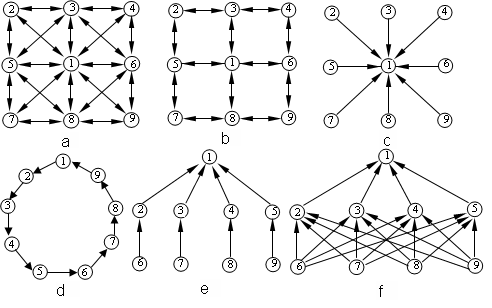
\includegraphics[width=\textwidth]{img/topology.png}
  \caption{Topológie paralelných genetických algoritmov \cite{pea}.}
  \label{img:topology}
\end{figure}

Schemy PGA
\subsection{Výsledky experimentu}
Vysledky PGA a ich interpretacia

%% Zaver
%%
%% Spolupraca s Petrom Javorkom
%% Spotrebovany cas/peniaze

